%____________________________________________________________________________
%
%STRUTTURA RELAZIONE:
%
%istituto
%scopo
%introduzione teorica
%strumentazione
%procedimento     
%dati sperimentali con tab
%elaborazione dati
%conclusione
%
%_____________________________________________________________________________

%NOTA UTILE: se in un testo bisogna inserire qualche dato numerico in riga, senza
%dover ricorrere a \begin{equation}, basta includere cio' che serve dentro a $....$
%esempio: $10k\Omega$ per inserire il dato in Ohm, poichè alcuni caratteri non vengono presi se stanno fuori da un'equazione


\documentclass{article}
\usepackage{amsmath}
\usepackage{setspace}
\usepackage{anysize}
\usepackage{geometry}
\usepackage{epsfig}
\usepackage{graphicx}
%c'è 1 inch di margine a destra e sinistra
%\geometry{margin = 1.25 in}

\title{\huge Relazione seconda esperienza di laboratorio \par Fisica 2}
\author{Gruppo A15: Armani Stefano, Cappellaro Nicola, Pasquato Leonardo}
\date{07-11-2022}
\setlength{\parindent}{0cm}

\begin{document}
    %print sezione titolo
    \maketitle
    \rule{\linewidth}{0.1mm}

    \section{Scopo dell'esperienza}
    Lo scopo della seconda esperienza di laboratorio è stato quello di prendere confidenza
    con due dei principali strumenti utilizzabili nello studio di una rete circuitale:
    il generatore di forme d'onda e l'oscilloscopio.\par
    Per comprendere al meglio il loro funzionamento e l'utilizzo, sono stati applicati
    ad un semplice circuito RC, a cui sono state date in ingresso diverse forme d'onda e 
    sono state studiate le risposte della rete a tali ingressi grazie all'oscilloscopio. 
    
    \section{Cenni teorici}

    \section{Strumentazione}
    \begin{itemize}
        \item Breadboard con annessi morsetti serrafilo;
        \item Cavi con connettori a banana;
        \item Resistori di varie misure ($1k\Omega$, $10k\Omega$, $100k\Omega$);
        \item Capacitori da $10nF$, $100nF$;
        \item Connettori da banco (Jumper);
        \item Generatore di forme d'onda Rigol DG1032;
        \item Oscilloscopio Rigol MSO2102A.
    \end{itemize}

    \section{Esperimento}
    
    Durante la prima parte di questa esperienza di laboratorio sono stati illustrati due
    importanti strumenti da banco, ossia il generatore di forme d'onda e l'oscilloscopio. \par
    La presentazione del generatore di forme d'onda è consistita nel presentare le varie impostazione
    percorribili in funzione della forma d'onda che si desidera generare: ampiezza, frequenza, fase, offset
    sono i parametri principali che sono stati modulati durante l'esperienza per alcuni segnali notevoli,
    ossia la funzione gradino, sinusoide, l'impulso. \par
    Successivamente sono stati applicati questi due strumenti in un semplice circuito RC, composto da
    un resistore e un capacitore in serie, generatore di forme d'onda e oscilloscopio collegato in parallelo
    al capacitore, come in figura.

    %non è chiaro il perchè, ma il !h potrebbe far incazzare latex
    \begin{figure}[!h]
        \begin{center}
            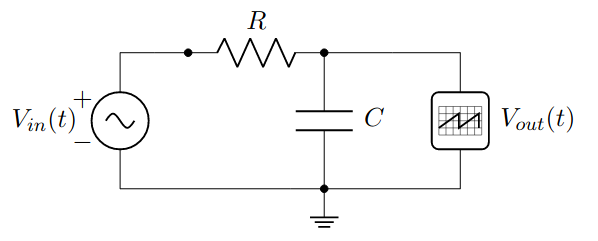
\includegraphics[width = 8cm]{circuito.png}
            \caption{Circuito RC}
        \end{center}
    \end{figure}
        
    Il primo esperimento è consistito nel dare in ingresso al circuito, per mezzo del generatore,
    un'onda quadra di frequenza $f = 10Hz$, tensione di picco $V_{In}^{pp} = 5V$ e offset nullo.\par
    Questo circuito è stato replicato 3 volte, con 3 diverse coppie di resistori e capacitori con diverse
    resistenze e capacità
    Grazie all'oscilloscopio è stato possibile ottenere il valore della tensione di lato ai capi 
    del capacitore in funzione del tempo, dunque sono stati ricavati dei valori di tensione istantanea,
    in momenti arbitrari, sia nella fase di carica che di scarica del capacitore.  \par
    Per questioni di semplicità, sono stati utilizzati i valori ottenuti dalla scarica del condensatore, in modo tale
    da poter stimare grazie al metodo della regressione lineare l'andamento della tensione.\par
    Ottenuti i valori delle costanti di tempo caratteristiche per ogni coppia di resistenze e capacità ($\tau$),
    è stato cambiato l'ingresso al circuito: il generatore di forme d'onda è stato impostato in modo tale da generare
    un'onda impulsiva. Ovviamente l'impulso, non replicabile nella realtà, è stato concretizzato in un'onda quadra di breve
    durata. \par
    La stessa procedura per ottenere i valori di tensioni istantanee è stata applicata anche in questo caso,
    al fine di studiare l'andamento della tensione avendo in ingresso un'onda impulsiva.
    L'ingresso impulsivo è stato modulato 3 volte, variando la durata dello stesso.
    L'onda quadra con durata minore delle 3 sarà sicuramente l'ingresso più approssimabile a quello impulsivo. \par
    

    \section{Dati sperimentali}
    \begin{center}
        Primo caso: \par
        R=$10k\Omega$ C=$100nF$
    \end{center}
    \begin{center}
    \begin{tabular}{|c|c|c|}
        \hline
        \textit{Test} & \textit{Tempo [us]} & \textit{Tensione [V]} \\
        \hline
        1 & 120 & 4.5 \\
        \hline
        2 & 360 & 3.54 \\
        \hline
        3 & 960 & 2.56 \\
        \hline
        4 & 1160 & 1.54 \\
        \hline
        5 & 2160 & 0.54 \\
        \hline
    \end{tabular}
    \end{center}
    
    \begin{center}
        Secondo caso: \par
        R=$10k\Omega$ C=$10nF$
    \end{center}
    \begin{center}
    \begin{tabular}{|c|c|c|}
        \hline
        \textit{Test} & \textit{Tempo [us]} & \textit{Tensione [V]} \\
        \hline
        1 & 32 & 3.54 \\
        \hline
        2 & 96 & 1.96 \\
        \hline
        3 & 202 & 0.7 \\
        \hline
        4 & 302 & 0.28 \\
        \hline
    
    \end{tabular}
    \end{center}

    \begin{center}
        Terzo caso: \par
        R=$200k\Omega$ C=$5nF$
    \end{center}
    \begin{center}
    \begin{tabular}{|c|c|c|}
        \hline
        \textit{Test} & \textit{Tempo [us]} & \textit{Tensione [V]} \\
        \hline
        1 & 100 & 3.69 \\
        \hline
        2 & 300 & 2.919 \\
        \hline
        3 & 540 & 2.099 \\
        \hline
        4 & 980 & 1.263 \\
        \hline
        5 & 1860 & 0.459 \\
        \hline
    
    \end{tabular}
    \end{center}

    \section{Elaborazione dati}

    
    \section{Conclusione}
    
\end{document}